\section{Model fitting and likelihood analysis}\label{sec:fitting}

In this section we simulate the fitting of source models to
lightcurves in the presence of random and systematic errors.  We
generate mock data for three source models --- a crescent, a uniform
disc and a Gaussian disc --- and then fit each mock light curve to all
three source models. Parameter fitting and marginalising was done by
Markov-chain Monte Carlo (MCMC).

\begin{figure}
\centering
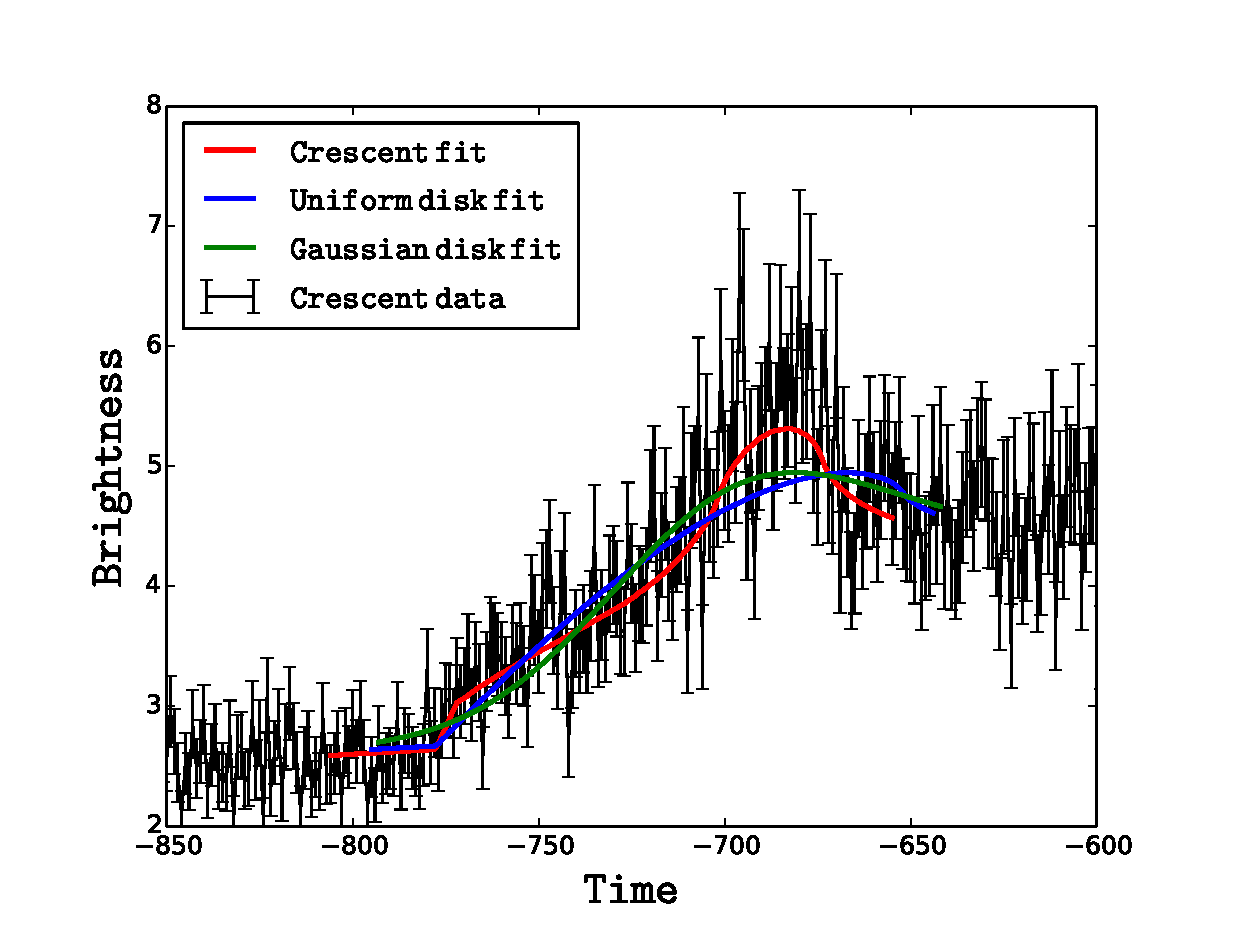
\includegraphics[width=0.9\hsize,bb=0 0 576 432
                ]{plots/data_cc.eps}
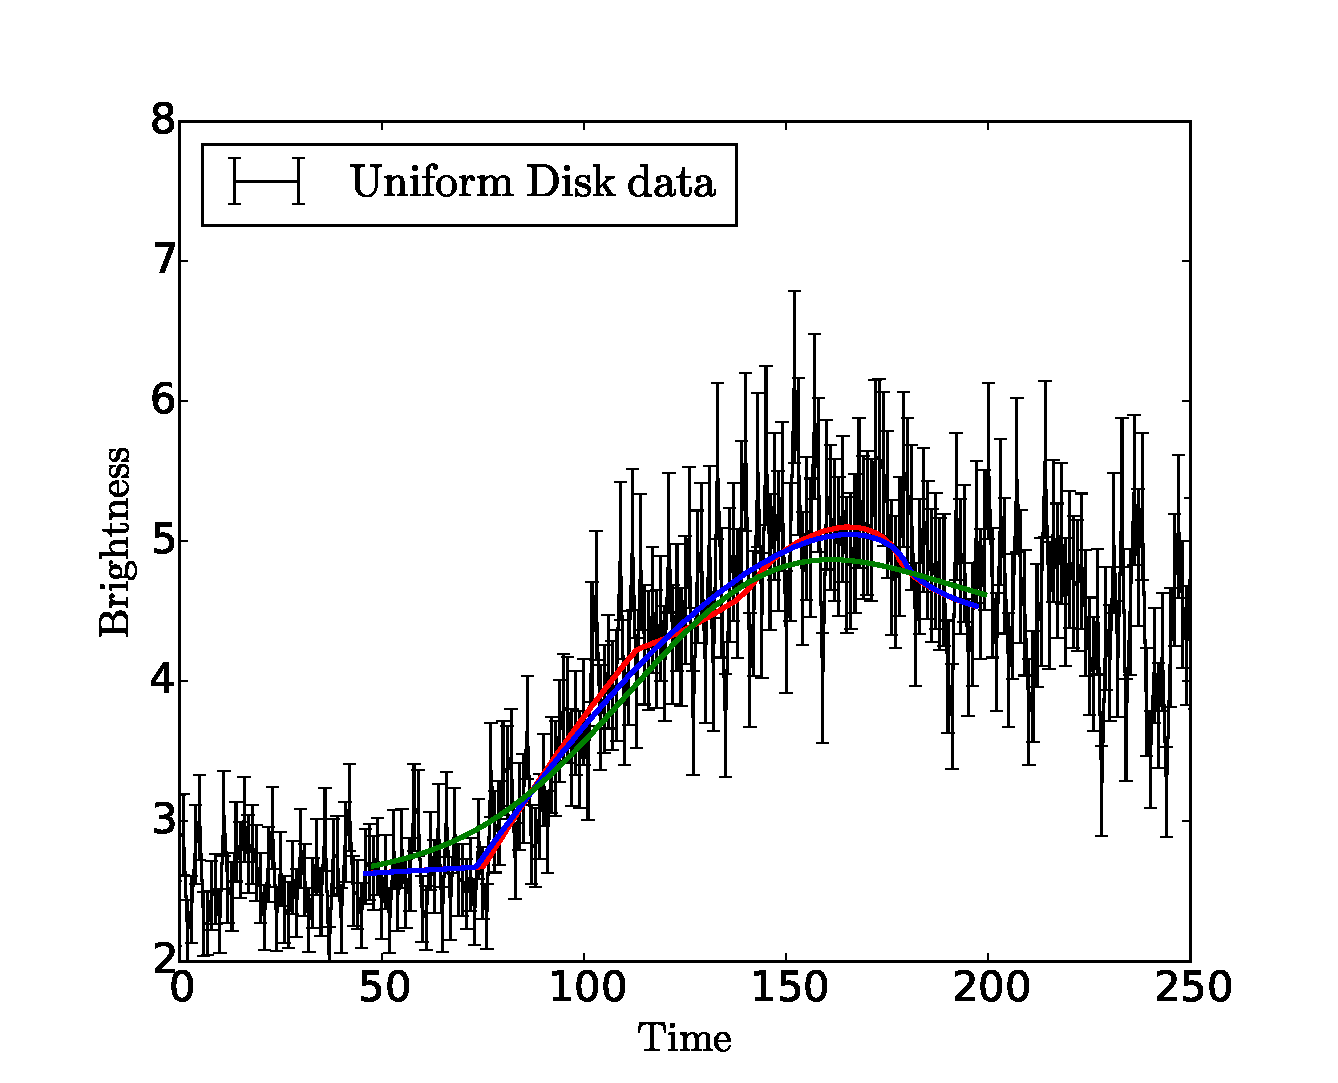
\includegraphics[width=0.9\hsize,bb=0 0 576 432
                ]{plots/data_dd.eps}
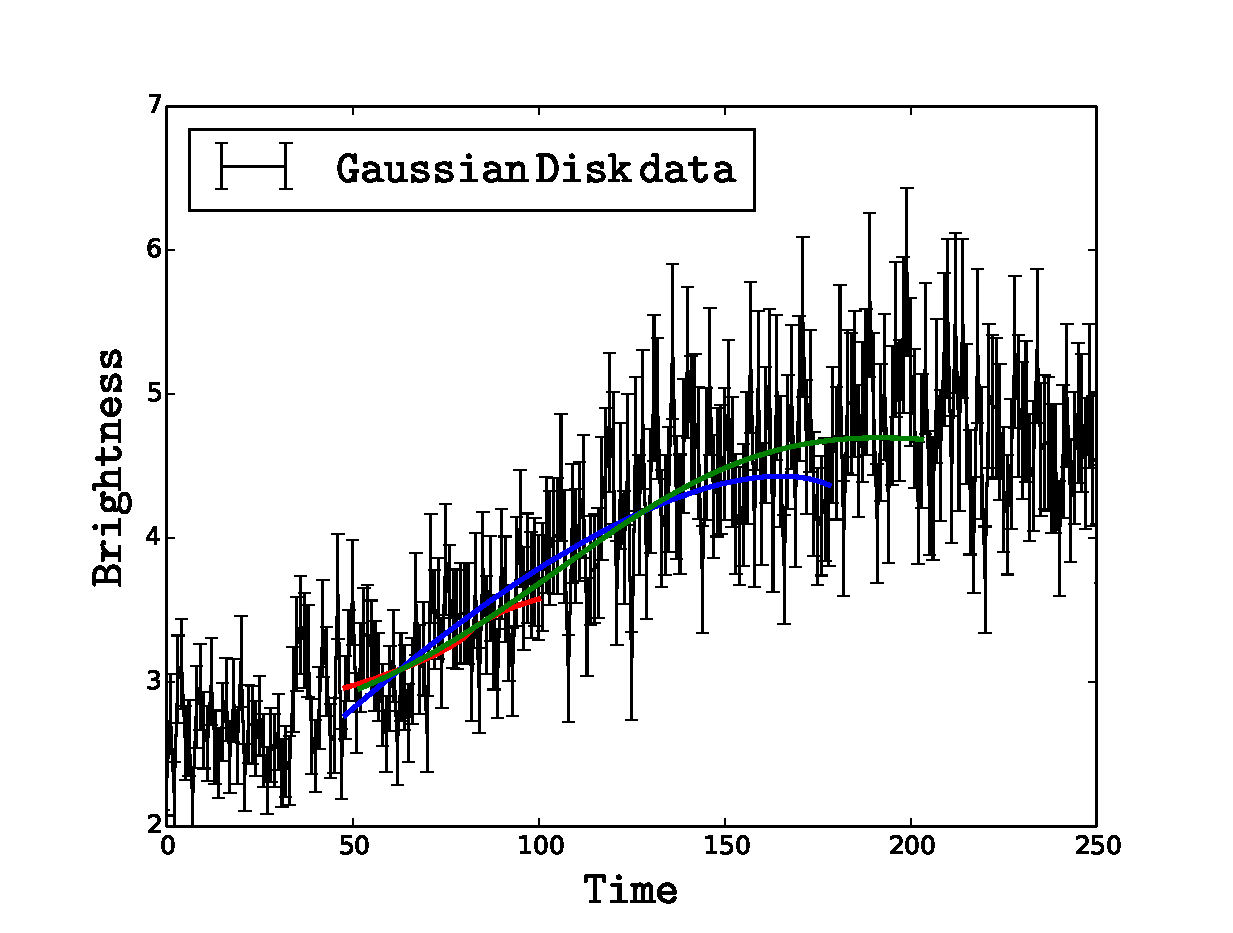
\includegraphics[width=0.9\hsize,bb=0 0 576 432
                ]{plots/data_gg.eps}
\caption{\label{fig:mockdata} Three different mock datasets with
  three different parametrizations fitted to each --- crescent (red),
  uniform-disk (blue) and Gaussian disk (green).}
\end{figure}

\subsection{Mock datasets}

Mock light curves were generated by running a source across a
caustic, specifically along the line from point C to point B in
Figure~\ref{fig:magnification_map}.  The model light curves, to which
these are fitted, are made by running a source across a different
caustic, along the line from point A to point B in the same figure.
That is, the mock data are generated with a clean but not ideal fold
caustic and then fitted with another such caustic.  This mimics the
unavoidable systematic error of not knowing the caustic exactly.

The crescent source had parameters (as explained in
\S\ref{subsec:crescent}) $R_p$ and $R_n$ being the radii of the outer
and inner circles and $(\alpha,\beta)$ being the coordinates of the inner
circle with respect to the centre of the outer circle in the coordinate system associated with the image in Figure 1 and not associated 
with the caustic surface as defined in the previous sections.  The parameter values were
\begin{equation}
   (R_p, R_n, $\alpha$, $\beta$) = (50.0, 30.0, 15.0, 10.0).
\label{eqn:cp}
\end{equation}
The uniform disc had the same (outer) radius as the crescent.  In the
Gaussian source, we set $3\sigma=50$.  For convenience, below we will
refer to $R_p$ of the Gaussian source, by which we actually mean
$3\sigma$.

Each mock light curve also has three nuisance parameters, namely the
beginning and end of the event and the brightness normalisation.
These are to be marginalised out by the MCMC.

Figure~\ref{fig:mockdata} shows the three light curves.  Each has
250 points regularly spaced in time, with Gaussian noise at the level
of 10\% of the current brightness.  The effective signal to noise can
be considered to be \textbf{ bad math here -- $0.1\times\sqrt{250}\simeq150$}.



\subsection{Fitting to mock data sets}

Each of the three mock light curves was fitted to all three models.
We denote the nine possible cases with letter pairs, with the first
letter denoting the assumed model for the fitting procedure and 
the second letter representing
the source: thus CG means a {\em C\/}rescent model was fitted to mock
data from a {\em G\/}aussian source, DC stands for a uniform {\em
  D\/}isc model fitted to mock data from a {\em C\/}rescent source,
and so on.

\begin{figure}
\centering
  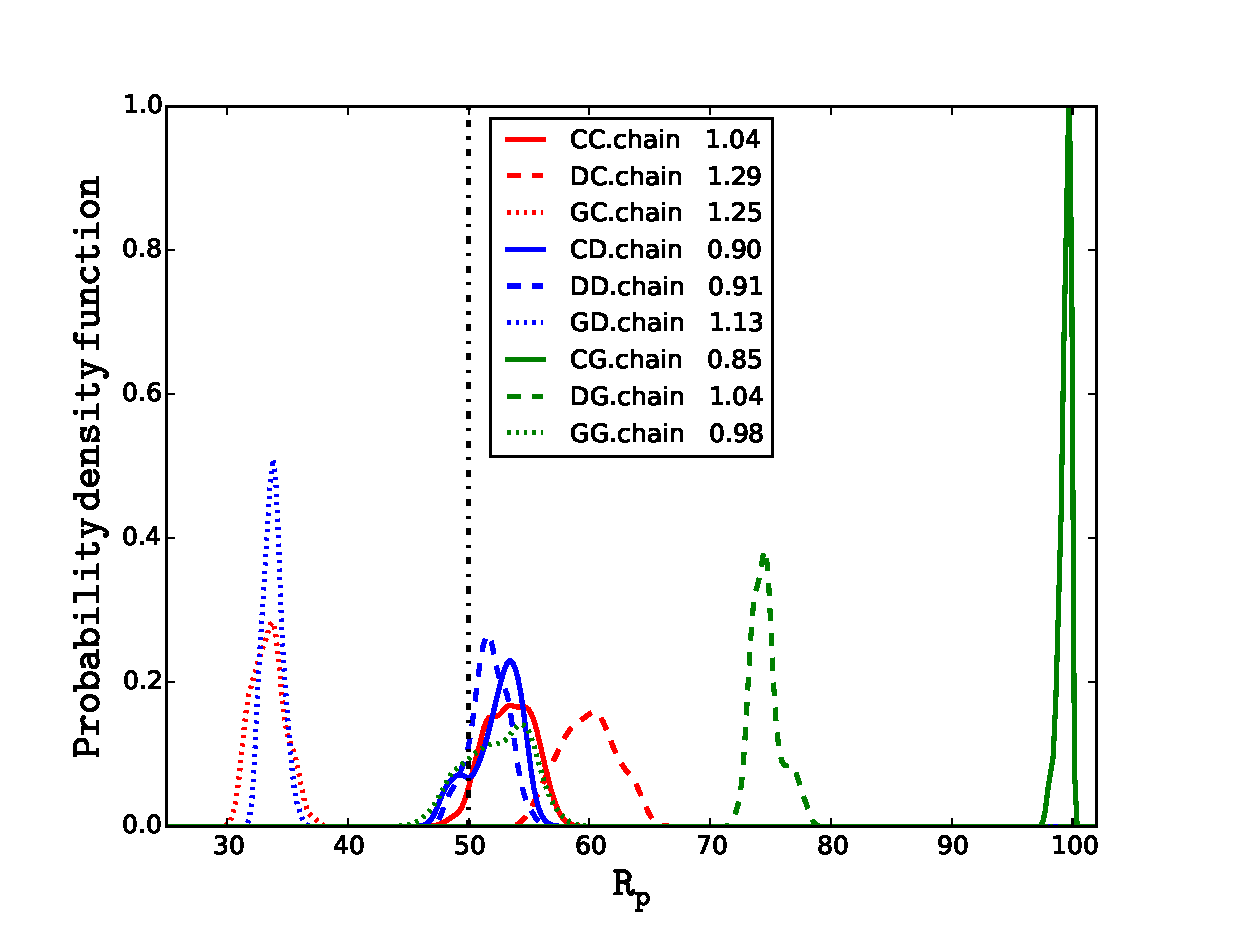
\includegraphics[width=0.9\hsize,bb=0 0 576 432
                  ]{plots/Rp4all.eps}
\caption{\label{fig:mcmc} Posterior probability distribution for the
  source size $R_p$.  The vertical line is the correct value. Same
  color represents the same dataset whereas same line style
  corresponds to same model fit.  The legend gives the reduced
  $\chi^2$ of the best fit in each case.}
\end{figure}

Figure~\ref{fig:mcmc} shows the posterior probability distribution of
$R_p$ for all nine cases, along with the minimum reduced $\chi^2$ for
each case.  The area under each curve is unity. Note that the height
of the curves are not the likelihood, they are probability densities
in parameter space.

\begin{figure}
\centering
  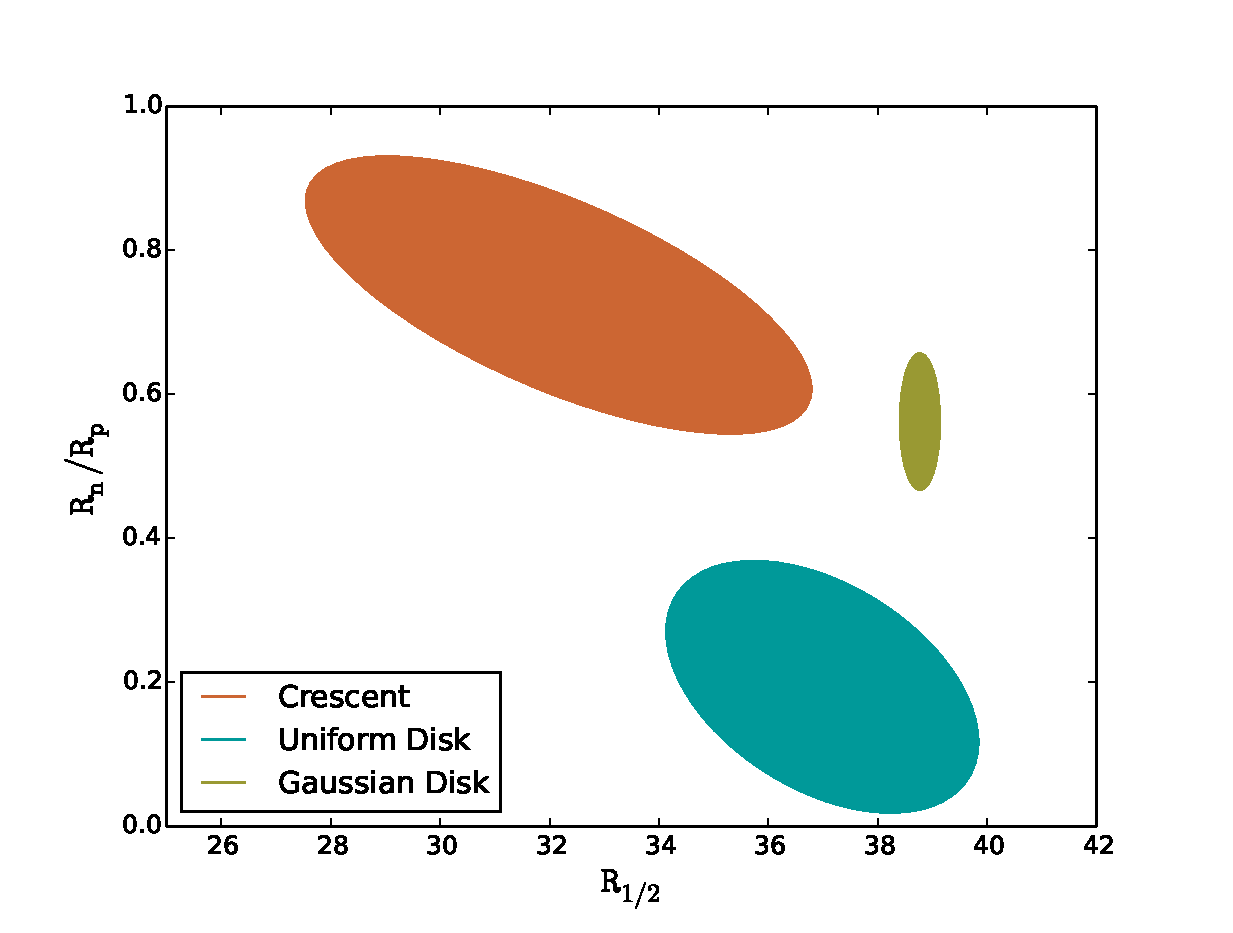
\includegraphics[width=0.9\hsize,bb=0 0 576 432
                  ]{plots/Rhalf_RnRp.eps}
  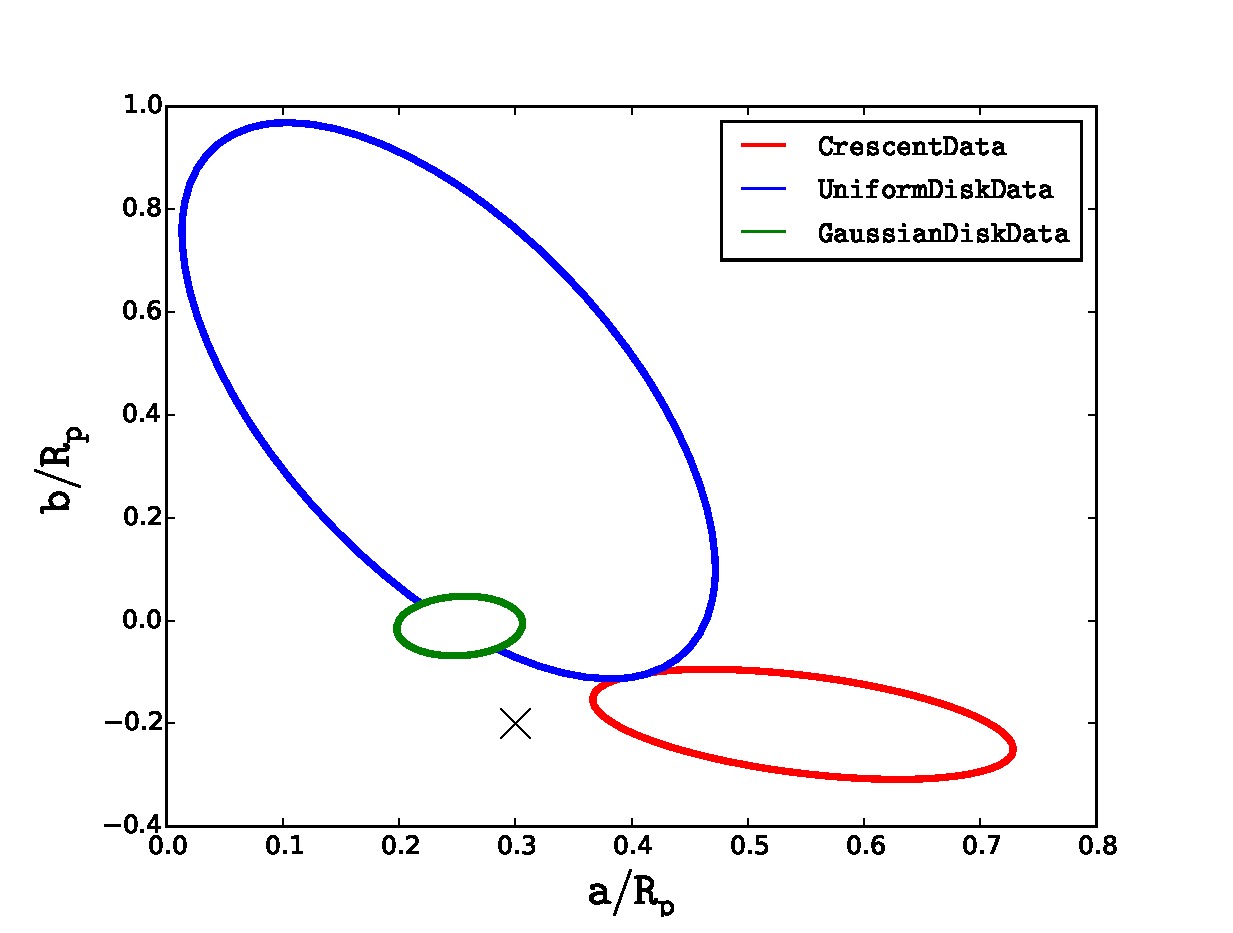
\includegraphics[width=0.9\hsize,bb=0 0 576 432
                  ]{plots/aRp_bRp.eps}
\caption{\label{fig:crescentfit} The 2$\sigma$ contours (or error ellipses)
  of the crescent model when fitting with the three different
  datasets.}
\end{figure}

Let us first consider the three cases where a crescent model was
fitted.  These are the solid curves in Figure~\ref{fig:mcmc}, with the
colours of the curves indicating the source.  Meanwhile,
Figure~\ref{fig:crescentfit} shows $2\sigma$ of the inferred parameter
values. \textbf{In the following enumerated conclusions we associate the word "wrong"
with parameters for which the real value corresponds to a PDF of the fitted model smaller than 
0.01. }

\begin{enumerate}

\item[1) {\bf CC}:] solid red curve in Figure~\ref{fig:mcmc} and red
  ellipses in Figure~\ref{fig:crescentfit}.  In this case, a light
  curve from a crescent source was being fitted to a crescent model.
  The fit gives reduced $\chi^2$ close to unity, as expected.  The
  recovered parameter values are near or slightly outside the
  $2\sigma$ ellipses.  This is expected, since we added a small
  systematic error, by using different caustics (though both clean
  folds) for the mock data and the model fit.  The apparent degeneracy
  between $a$ and $b$, seen in Figure~\ref{fig:crescentfit}, is also
  expected, since only the distance of the crescent's small circle
  from the caustic influences the magnification.


\item[2) {\bf CD}:] solid blue curve and blue ellipses.  Here a
  crescent model was fitted to a light curve from a uniform disc.  The
  situation is formally a crescent with $R_n=0$ and $a,b$ arbitrary,
  and this shows in the blue ellipses in the recovered parameter
  values.  The redundant parameters $\alpha$ and $\beta$, in effect, allow the
  model to partly fit the noise, and hence the $\chi^2$ is somewhat
  lower than in the previous case.

\begin{figure}
\centering
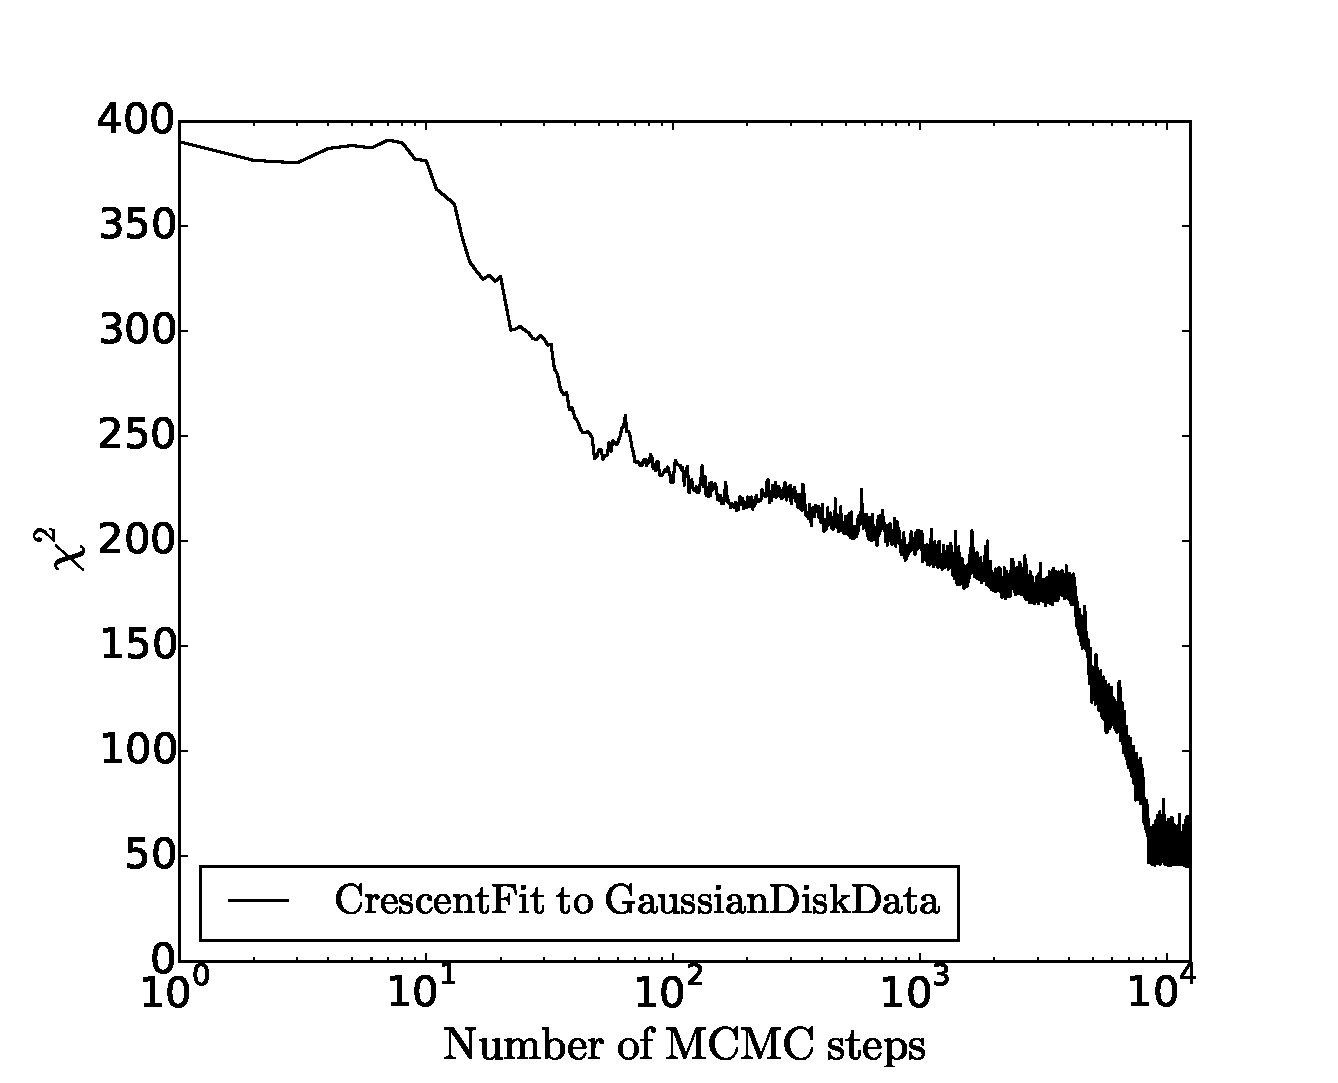
\includegraphics[width=0.9\hsize,bb=0 0 576 432
                ]{plots/burnin_cg.eps}
\caption{\label{fig:burnin} The $\chi^2$ of each step of the full MCMC
  for one case.}
\end{figure}

\item[3) {\bf CG}:] Solid green curve and green ellipses.
  Additionally, Figure~\ref{fig:burnin} shows the progress of
  reduction of $\chi^2$ in this case, where a crescent-source model is
  used to fit data from a Gaussian source.  The parameter values are
  seemingly tightly constrained, but the recovered $R_p$ is completely
  wrong.  The reduced $\chi^2$ is only 0.85, indicative of
  over-fitting.  We can see what has happened from the red curve in
  the bottom panel of Figure~\ref{fig:mockdata}.  The best-fit model
  covers only a small part of the light curve.  That is, the fitting
  procedure has exploited the nuisance parameters to find a good fit
  to mainly noise.

\end{enumerate}

Next we consider the three cases where a disc model is fitted.  These
correspond to the dashed curves in Figure~\ref{fig:mcmc}.  There is
only one interesting parameter to fit, the disc radius $R_p$, and no
equivalent of Figure~\ref{fig:crescentfit} is needed. 

\begin{enumerate}

\item[4) {\bf DC}:] red dashed curve.  On fitting a disc model to a
  crescent-source source, the recovered $R_p$ is incorrect, but the
  reduced $\chi^2$ of 1.29 signals that the data reject the model.

\item[5) {\bf DD}:] red dashed curve.  When the correct model is
  fitted to a disc-source, the best fit $\chi^2=0.91$ is good and
  $R_p$ is recovered within the uncertainty estimate.

\item[6) {\bf DG}:] green dashed curve.  On fitting a disc model to a
  Gaussian-source model, the recovered $R_p$ is incorrect, but the
  reduced $\chi^2$ gives no signal that something is amiss.  It
  appears that a Gaussian source could mimic a uniform disc.

\end{enumerate}

Finally, we consider the three cases where a Gaussian model is fitted.
These correspond to the dotted curves in Figure~\ref{fig:mcmc}.  Again,
there is only one interesting parameter to fit, the Gaussian
$3\sigma$-radius, which we have called $R_p$.

\begin{enumerate}

\item[7) {\bf GC}:] red dotted curve.  When a Gaussian-source model is
  fitted to data from a crescent source, the recovered $R_p$ is wrong
  but the reduced $\chi^2=1.29$ shows the data rejecting the model.

\item[8) {\bf GD}:] blue dotted curve.  When a Gaussian-source model
  is fitted to data from a uniform disc, the recovered $R_p$ is wrong
  but the model is rejected anyway.

\item[9) {\bf GG}:] green dotted curve.  When data from a Gaussian is
  fitted to the correct model, $R_p$ is recovered within its estimated
  uncertainty, and the best fit reduced $\chi^2$ is close to unity.

\end{enumerate}

The above results suggest the following strategy for fitting a
lightcurve from an unknown source profile: first try a Gaussian-source
model; if the data reject that model, try a uniform disc; if the
uniform disc is also rejected by the data, try a crescent model.  Our
numerical experiments indicate --- assuming one of the three source
models is correct --- that the reduced $\chi^2$ would unmask the
correct model, \textbf{and its parameters would be correctly recovered}.

